
\begin{frame}{Implementation}
    \begin{columns}
        \begin{column}{0.5\linewidth}
            \vspace*{-1mm}
            \begin{itemize}
                \item \textbf{Language}: Python 3.14
                \item \textbf{Library}: \texttt{mclbn256}
                \item \textbf{Architecture}: Multi-process 
                \item \textbf{Communication}: UDP sockets
            \end{itemize}
            \vfill
            \begin{figure}
                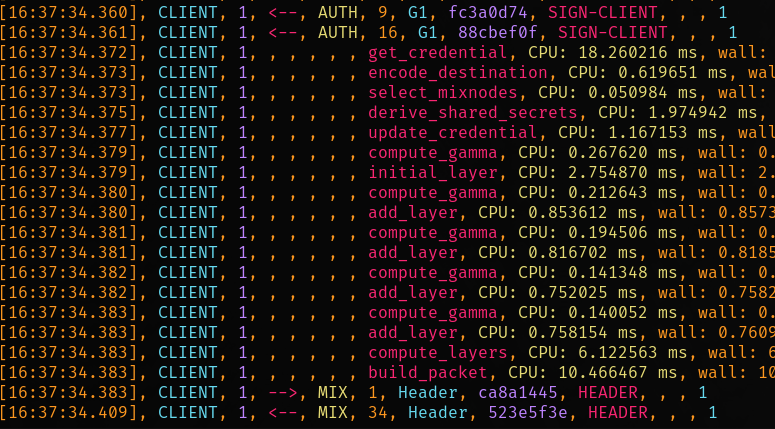
\includegraphics[width=0.95\linewidth]{schema/script_2.png}
                \vspace*{-3mm}
                \caption{Log files}
            \end{figure}
        \end{column}
        \begin{column}{0.5\linewidth}
            \vspace*{-2mm}
            \begin{figure}
                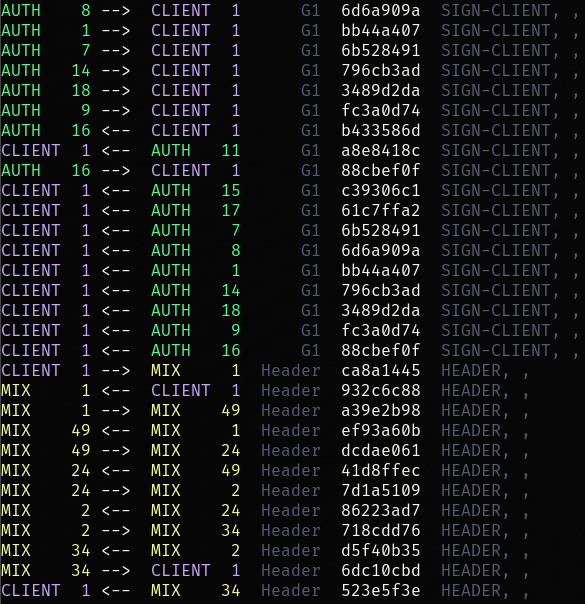
\includegraphics[width=0.85\linewidth]{schema/script_1.png}
                \vspace*{-3mm}
                \caption{Script running}
            \end{figure} 
        \end{column}
    \end{columns}
\end{frame}

\begin{frame}{Results: Scaling degree on CPU time execution for each functions}
    \begin{figure}
        \vspace*{-2mm}
        
\includegraphics[scale=0.3]{schema/CPU_scaling.png}
    \end{figure} 
\end{frame}

\begin{frame}{Results: Latency Comparison with Sphinx Baseline}
    \begin{figure}
        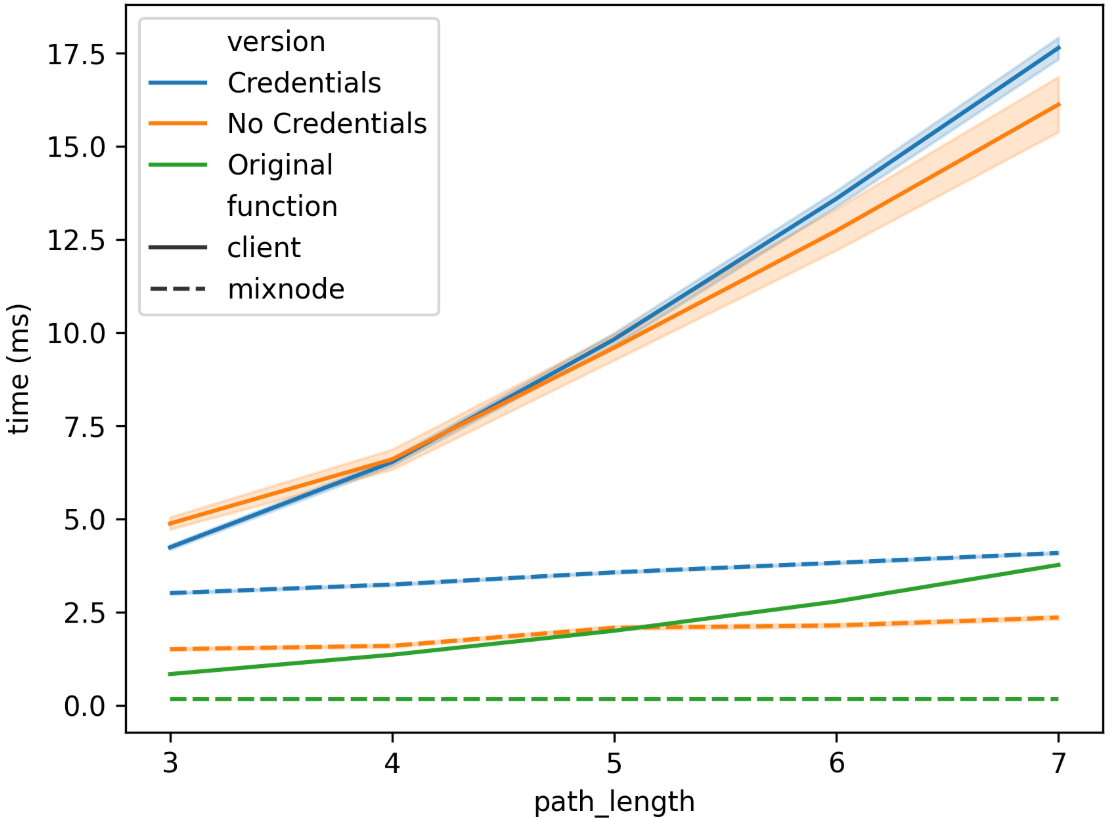
\includegraphics[width=0.65\linewidth]{schema/run_time.png}
        \vspace*{-3mm}
        \caption{Script running}
    \end{figure} 
\end{frame}